%#!uplatex main.tex

\section{Application}

In this section, we introduce advanced usage of IIS.

\subsection{Render internal area}

\begin{figure}[htbp]
  \center
  \includegraphics[height=1.35in, keepaspectratio]{img/application/internal/schottky.png}
  \caption{\textit{Edge of the circlte inversion fractal}}
  \label{fig:divideTwo}
 \hspace*{\fill}
\end{figure}

%% 二次元のフラクタルの内側だけを描く.全ての円盤が接していれば極限集合
%% で二分割することができる

In two dimensional circle inversion fractals,
when all of the circles touches each other, the limit set divides plane
into two. See Figure \ref{fig:divideTwo}.
transformed point is outside of the limit set.

We fill a pixel result of IIS, the point moved into inner part of the
resulting fractal.

\subsection{Render Edge of the Circles}

\begin{figure}[htbp]
  \center
  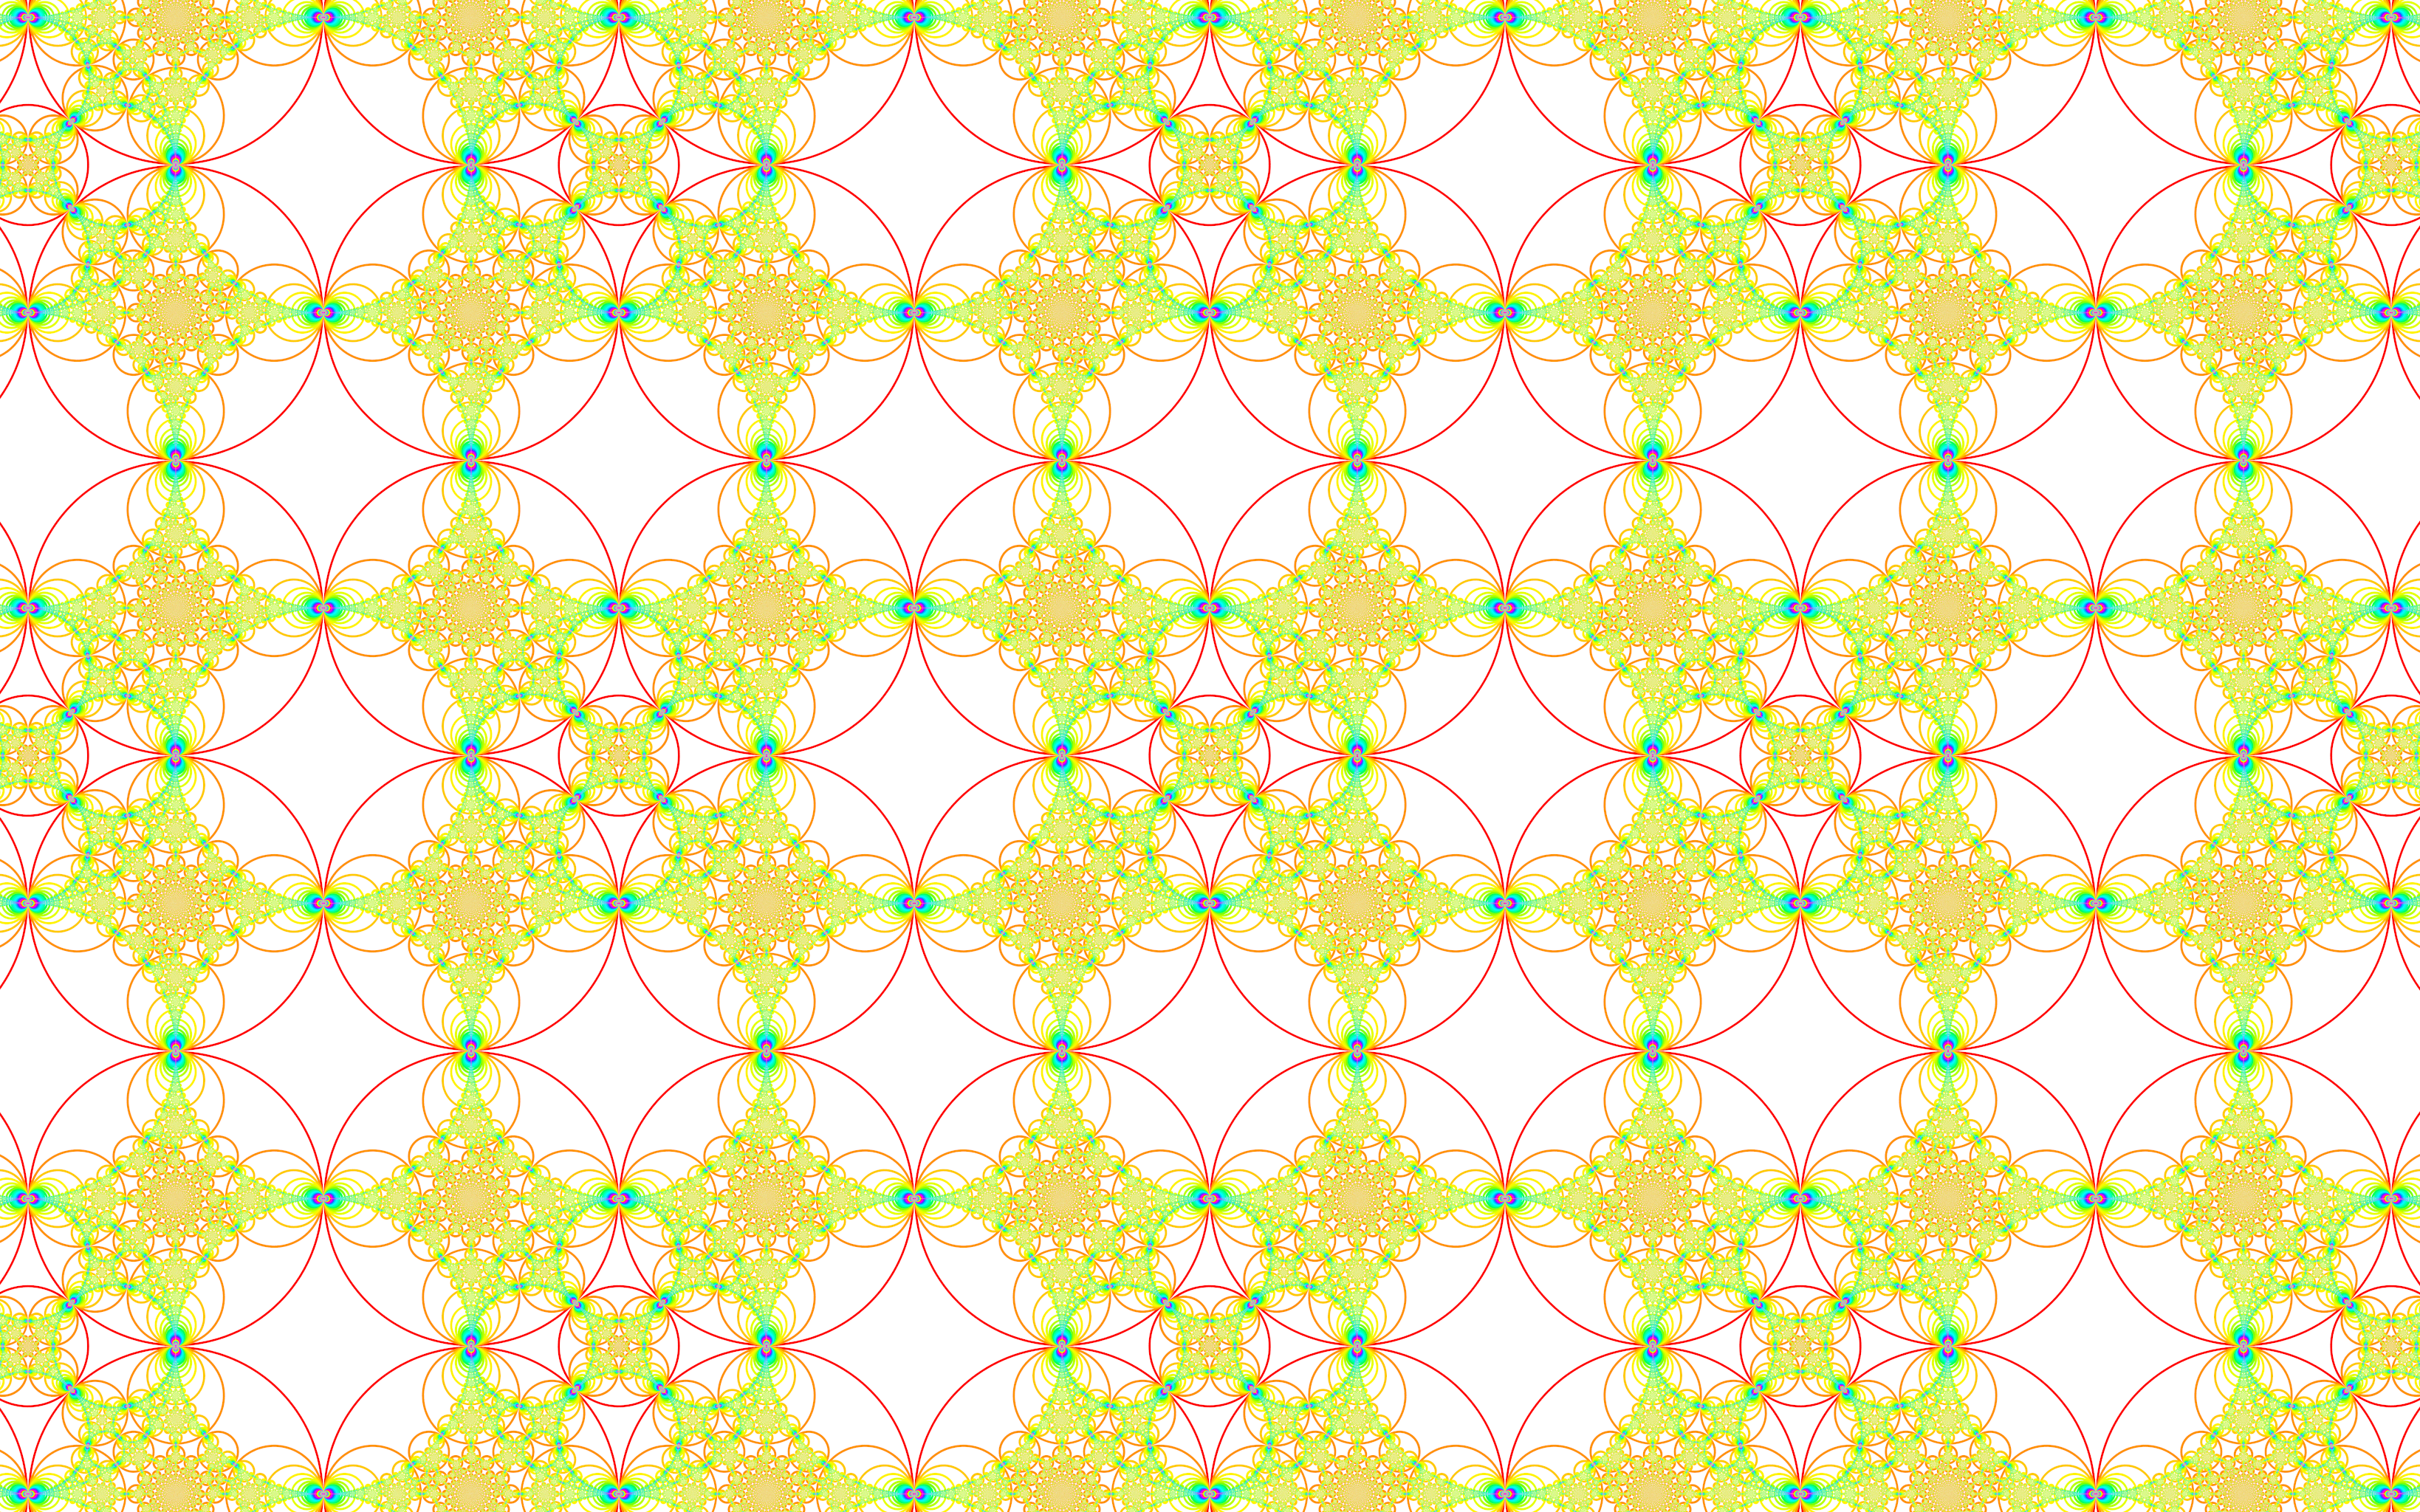
\includegraphics[height=1.35in, keepaspectratio]{img/application/edge/circleEdge.png}
  \caption{\textit{Edge of the circlte inversion fractal}}
  \label{fig:circleEdge}
 \hspace*{\fill}
\end{figure}

We can draw only edges of disks in circle inversion fractals.
We can estimate the distance from the center of the disks using jacobian
of circle inversions.

%% ヤコビアンを累積させていき,最後の円周からの距離を累積させたヤコビア
%% ンで割ることで,円周から点までの距離を得ることができる.

\subsection{Geometrical Representation of M\"obius Transformation Groups}

%% メビウス変換を円や球の反転で定義することによって,より直観的に生成元
%% を得て描画することができる.

In this paper, we mainly use circle or sphere inversions.
We can compose M\"obius transformations by even number of
inversion.
So far, we only use simple circle or sphere inversions.
Other interesting images can be generated using more
complicated M\"obius transformations.
It is known that we can construct any M\"obius transformation out of
inversions.
Thus, we can apply IIS to visualize fractals combining circle inversion
fractals and M\"obius transformation groups.
Moreover, we can tweak parameters of M\"obius transformations by
arranging geometrical objects like circles or lines on the plane.

\subsubsection{Two Dimensionanl Generators}

\begin{figure}[htbp]
 \begin{minipage}[t]{0.5\hsize}
  \begin{minipage}{0.25\hsize}
   \center
   \includegraphics[ height=1.4in, keepaspectratio]{./img/application/2dGen/infInvEdgedGen.pdf}
   \subcaption{\textit{Generator}}
   \label{fig:infCircleGen}
  \end{minipage}
  \hspace*{\fill}
  \begin{minipage}{0.25\hsize}
   \center
   \includegraphics[ height=1.4in, keepaspectratio]{./img/application/2dGen/infInvEdgedOrb.pdf}
   \subcaption{\textit{Orbit}}
   \label{fig:infCircleOrb}
  \end{minipage}
  \hspace*{\fill}
  \caption{\textit{Inversion in the circle with \\ infinite radius and
  four Schottky disks}}
  \label{fig:infCircle}
 \end{minipage}
 \begin{minipage}[t]{0.5\hsize}
  \begin{minipage}{0.25\hsize}
   \center
   \includegraphics[ height=1.4in, keepaspectratio]{./img/application/2dGen/translationEdgedGen.pdf}
   \subcaption{\textit{Generator}}
   \label{fig:translation2dGen}
  \end{minipage}
  \hspace*{\fill}
  \begin{minipage}{0.25\hsize}
   \center
   \includegraphics[ height=1.4in, keepaspectratio]{./img/application/2dGen/translationEdgedOrb.pdf}
   \subcaption{\textit{Orbit}}
   \label{fig:translation2dOrb}
  \end{minipage}
  \hspace*{\fill}
  \caption{\textit{Parallel translation generator and four Schottky disks}}
  \label{fig:translation2d}
 \end{minipage}
 \end{figure}

\begin{figure}[htbp]
 \begin{minipage}{0.5\hsize}
  \begin{minipage}{0.25\hsize}
   \center
   \includegraphics[ height=1.4in, keepaspectratio]{./img/application/2dGen/rotationEdgedGen.pdf}
   \subcaption{\textit{Generator}}
   \label{fig:rotation2dGen}
  \end{minipage}
 \hspace*{\fill}
  \begin{minipage}{0.25\hsize}
   \center
   \includegraphics[ height=1.4in, keepaspectratio]{./img/application/2dGen/rotationEdgedOrb.pdf}
   \subcaption{\textit{Orbit}}
   \label{fig:rotation2dOrb}
  \end{minipage}
  \hspace*{\fill}
  \caption{\textit{Rotation generator and three Schottky disks}}
  \label{fig:Rotation2d}
 \end{minipage}
 \begin{minipage}{0.5\hsize}
  \begin{minipage}{0.25\hsize}
   \center
   \includegraphics[ height=1.4in, keepaspectratio]{./img/application/2dGen/hyperbolicRect0.pdf}
   \subcaption{\textit{Generator}}
   \label{fig:hyperbolic2dGen}
  \end{minipage}
 \hspace*{\fill}
  \begin{minipage}{0.25\hsize}
   \center
   \includegraphics[ height=1.4in, keepaspectratio]{./img/application/2dGen/hyperbolicRect.pdf}
   \subcaption{\textit{Orbit}}
   \label{fig:hyperbolic2dOrb}
  \end{minipage}
 \hspace*{\fill}
  \caption{\textit{Hyperbolic generator and a Schottky disk}}
  \label{}
 \end{minipage}
\end{figure}

\begin{figure}[htbp]
 \begin{minipage}[t]{0.5\hsize}
  \begin{minipage}{0.25\hsize}
   \center
   \includegraphics[ height=1.4in, keepaspectratio]{./img/application/2dGen/parabolicRect0.pdf}
   \subcaption{\textit{Generator}}
   \label{fig:parabolic2dGen}
  \end{minipage}
 \hspace*{\fill}
  \begin{minipage}{0.25\hsize}
   \center
   \includegraphics[ height=1.4in, keepaspectratio]{./img/application/2dGen/parabolicRect.pdf}
   \subcaption{\textit{Orbit}}
   \label{fig:parabolic2dOrb}
  \end{minipage}
  \hspace*{\fill}
  \caption{\textit{The orbit of Parabolic generator and \\a Schottky disk}}
  \label{fig:parabolic2d}
 \end{minipage}
 \begin{minipage}[t]{0.5\hsize}
  \begin{minipage}{0.25\hsize}
   \center
   \includegraphics[ height=1.4in, keepaspectratio]{./img/application/2dGen/loxo0.pdf}
   \subcaption{\textit{Generator}}
   \label{fig:loxo2dGen}
  \end{minipage}
 \hspace*{\fill}
  \begin{minipage}{0.25\hsize}
   \center
   \includegraphics[ height=1.4in, keepaspectratio]{./img/application/2dGen/loxoOrb.pdf}
   \subcaption{\textit{Orbit}}
   \label{fig:loxo2dOrb}
  \end{minipage}
 \hspace*{\fill}
  \caption{\textit{Loxodromic generator and a Schottky disk}}
  \label{fig:loxodromic2d}
 \end{minipage}
\end{figure}

\noindent\textbf{Inversion in a Circle with Infinite Radius.}
An inversion in a circle with infinite radius is treated as a reflection
over a border line of half plane. See Figure
\ref{fig:infCircle}\subref{fig:infCircleGen}.
The four inversion circles are lying on the right side, and there is the
orange region on the left side. The region is is a half plane, that is, a
disk with infinite radius. Its boundary is colored with white line.
The orbit is shown in
Figure \ref{fig:infCircle}\subref{fig:infCircleOrb}.
As we can see, the circles are reflected over the white line.

\noindent\textbf{Parallel Translation.}
A composition of reflections over two parallel half planes facing each
other generates a parallel translation. See Figure
\ref{fig:translation2d}\subref{fig:translation2dGen}.
There are two orange half planes on the right and left sides.
The orbit is shown in Figure
\ref{fig:translation2d}\subref{fig:translation2dOrb}.

\noindent\textbf{Rotation.}
A composition of reflections over two crossing half planes generates a
rotation. The generator is shown in Figure
\ref{fig:Rotation2d}\subref{rotation2dGen}
The two half planes are crossing. The rotation axis is crossing point of
white border lines. The orbit is shown in Figure 
\ref{fig:Rotation2d}\subref{rotation2dOrb}.
It has a rotation symmetry and it is an elliptic transformation.

\noindent\textbf{Composition of Two Circles.}
%% Hyperbolic, parabolic, elliptic

\noindent\textbf{Loxodromic.}


\subsubsection{Three Dimensionanl Generators}

\begin{figure}[h!tbp]
 \begin{minipage}[t]{0.5\hsize}
  \begin{minipage}{0.25\hsize}
   \center
   \includegraphics[width=1.4in, height=1.4in, keepaspectratio]{./img/application/3dGen/infSphereGen.pdf}
   \subcaption{\textit{Generator}}
   \label{fig:infSphereGen}
  \end{minipage}
  \hspace*{\fill}
  \begin{minipage}{0.25\hsize}
   \center
   \includegraphics[width=1.4in, height=1.4in, keepaspectratio]{./img/application/3dGen/infSphereOrbit.pdf}
   \subcaption{\textit{Orbit}}
   \label{fig:infSphereOrb}
  \end{minipage}
  \hspace*{\fill}
  \caption{\textit{Inversion in the sphere with infinite radius, four
  Schottky spheres, and a base sphere}}
  \label{fig:infSphere}
 \end{minipage}
 \hspace*{\fill}
 \begin{minipage}[t]{0.5\hsize}
  \begin{minipage}{0.25\hsize}
   \center
   \includegraphics[width=1.4in, height=1.4in, keepaspectratio]{./img/application/3dGen/translationGen.pdf}
   \subcaption{\textit{Generator}}
   \label{fig:translation3dGen}
  \end{minipage}
  \hspace*{\fill}
 \begin{minipage}{0.25\hsize}
  \center
  \includegraphics[width=1.4in, height=1.4in, keepaspectratio]{./img/application/3dGen/translationOrbit.pdf}
  \subcaption{\textit{Orbit}}
    \label{fig:translation3dOrb}
 \end{minipage}
  \hspace*{\fill}
  \caption{\textit{Parallel translation generator, six Schottky spheres
  and a base sphere}}
  \label{fig:translation3d}
 \end{minipage}
\end{figure}

\begin{figure}[h!tbp]
 \begin{minipage}[t]{0.5\hsize}
  \begin{minipage}{0.25\hsize}
   \center
    \includegraphics[width=1.4in, height=1.4in, keepaspectratio]{./img/application/3dGen/compParabolicGen.pdf}
    \subcaption{\textit{Generator}}
    \label{fig:compParabolicGen}
  \end{minipage}
  \hspace*{\fill}
  \begin{minipage}{0.25\hsize}
   \center
   \includegraphics[width=1.4in, height=1.4in, keepaspectratio]{./img/application/3dGen/compParabolicOrb.pdf}
   \subcaption{\textit{Orbit}}
   \label{fig:compParabolicOrb}
  \end{minipage}
  \hspace*{\fill}
  \caption{\textit{Compound parabolic generator, six \\Schottky spheres
  and a base sphere}}
  \label{fig:compParabolic}
 \end{minipage}
 \hspace*{\fill}
 \begin{minipage}[t]{0.5\hsize}
  \begin{minipage}{0.25\hsize}
   \center
   \includegraphics[width=1.4in, height=1.4in, keepaspectratio]{./img/application/3dGen/rotationGen.pdf}
   \subcaption{\textit{Generator}}
   \label{fig:rotationGen}
  \end{minipage}
  \hspace*{\fill}
  \begin{minipage}{0.25\hsize}
   \center
   \includegraphics[width=1.4in, height=1.4in, keepaspectratio]{./img/application/3dGen/rotationOrb.pdf}
   \subcaption{\textit{Orbit}}
   \label{fig:rotationOrb}
  \end{minipage}
  \hspace*{\fill}
  \caption{\textit{Rotation generator, four Schottky spheres, and a base
  sphere}}
  \label{fig:rotation3d}
 \end{minipage}
\end{figure}

\begin{figure}[h!tbp]
 \begin{minipage}{0.5\hsize}
  \begin{minipage}{0.25\hsize}
   \center
   \includegraphics[width=1.4in, height=1.4in, keepaspectratio]{./img/application/3dGen/loxoGenSimple.pdf}
   \subcaption{\textit{Generator}}
   \label{fig:loxoGen3d}
  \end{minipage}
  \hspace*{\fill}
  \begin{minipage}{0.25\hsize}
   \center
   \includegraphics[width=1.4in, height=1.4in, keepaspectratio]{./img/application/3dGen/loxoOrbSimple.pdf}
   \subcaption{\textit{Orbit}}
   \label{fig:loxoOrb3d}
  \end{minipage}
  \hspace*{\fill}
 \caption{\textit{Hyperbolic generator and a base sphere}}
  \label{fig:loxo3d}
 \end{minipage}
 \hspace*{\fill}
 \begin{minipage}{0.5\hsize}
  \begin{minipage}{0.25\hsize}
   \center
   \includegraphics[width=1.4in, height=1.4in, keepaspectratio]{./img/application/3dGen/parabolicOneGen.pdf}
   \subcaption{\textit{Generator}}
   \label{fig:parabolic3dGen}
  \end{minipage}
  \hspace*{\fill}
  \begin{minipage}{0.25\hsize}
   \center
   \includegraphics[width=1.4in, height=1.4in, keepaspectratio]{./img/application/3dGen/parabolicOneOrb.pdf}
  \subcaption{\textit{Orbit}}
   \label{fig:parabolic3dOrb}
  \end{minipage}
  \hspace*{\fill}
  \caption{\textit{Parabolic generator and a base sphere}}
  \label{fig:parabolic3d}
 \end{minipage}
\end{figure}

\begin{figure}[h!tbp]
 \begin{minipage}[t]{0.5\hsize}
  \begin{minipage}[t]{0.25\hsize}
   \center
   \includegraphics[width=1.4in, height=1.4in, keepaspectratio]{./img/application/3dGen/loxoOrbSch.pdf}
   \subcaption{\textit{Hyperbolic}}
  \end{minipage}
  \hspace*{\fill}
  \begin{minipage}[t]{0.25\hsize}
   \center
   \includegraphics[width=1.4in, height=1.4in, keepaspectratio]{./img/application/3dGen/parabolicOrb.pdf}
   \subcaption{\textit{Parabolic}}
  \end{minipage}
  \hspace*{\fill}
  \caption{\textit{The orbit generated by a composition \\of two spheres and six Schottky
  spheres}}
  \label{fig:complicated3d}
 \end{minipage}
 \hspace*{\fill}
 \begin{minipage}[t]{0.5\hsize}
  \begin{minipage}[t]{0.25\hsize}
   \center
   \includegraphics[width=1.4in, height=1.4in, keepaspectratio]{./img/application/3dGen/compLoxoOneGen.pdf}
   \subcaption{\textit{Generator}}
   \label{fig:compLoxoGen}
  \end{minipage}
 \hspace*{\fill}
  \begin{minipage}[t]{0.25\hsize}
   \center
   \includegraphics[width=1.4in, height=1.4in, keepaspectratio]{./img/application/3dGen/compLoxoOneOrb.pdf}
   \subcaption{\textit{Orbit}}
   \label{fig:compLoxoOrb}
  \end{minipage}
  \hspace*{\fill}
  \caption{\textit{Compound loxodromic generator and a base sphere}}
  \label{fig:compLoxo}
 \end{minipage}
\end{figure}

\noindent\textbf{Inversion in a Sphere with Infinite Radius.}

\noindent\textbf{Parallel
Translation~\footnote{\url{https://www.shadertoy.com/view/lsjyzK}}.}

\noindent\textbf{Rotation.}

\noindent\textbf{Composition of Two
Spheres~\footnote{\url{https://www.shadertoy.com/view/ldByDW}}.}
%% Hyperbolic, parabolic, elliptic

\noindent\textbf{Compound Loxodromic~\footnote{\url{https://www.shadertoy.com/view/MdjyRV}}.}

\subsection{Sphairahedra and Three-dimensional Fractals}

%% 球面体のタイリングもIISで描画することができる

In 2003, Kazushi Ahara and Yoshiaki Araki invented
\textit{Sphairahedron} to introduce new kind of three dimensional
fractals \cite{ahara2003sphairahedral}.

Sphairahedron is coined word combining two words sphaira- and -hedron.

The fractals are generated by tiling of sphairahedra.

We use IIS for three dimensional tiling.
This method uses 
For more details, read \cite{bridges2018:171}